\subsection{Описание процесса управления адресной светодиодной лентой}
\label{sec:analysis:businessProccess}

Для того, чтобы воспользоваться всеми возможностями адресной светодиодной ленты, пользователь должен первоначально купить ее, установить ее в удобном месте, скачать описанное в записке программное обеспечение на мобильный телефон и провести процесс инициализации адресной ленты.

Функционирование украшения дома в данном проекте описаны с помощью функциональной модели IDEF0.

Для представления процессов, возникающих при приобретении и использовании адресных светодиодных лент (украшений) была разработана функциональная модель \enquote{Управлять адресной светодиодной лентой}. Процесс состоит из нескольких этапов, которые подробно описаны на рисунках~\ref{fig:analysis:functionalModel:main}~–~\ref{fig:analysis:functionalModel:a42_connecting}.

~
\begin{figure}[H]
\centering
	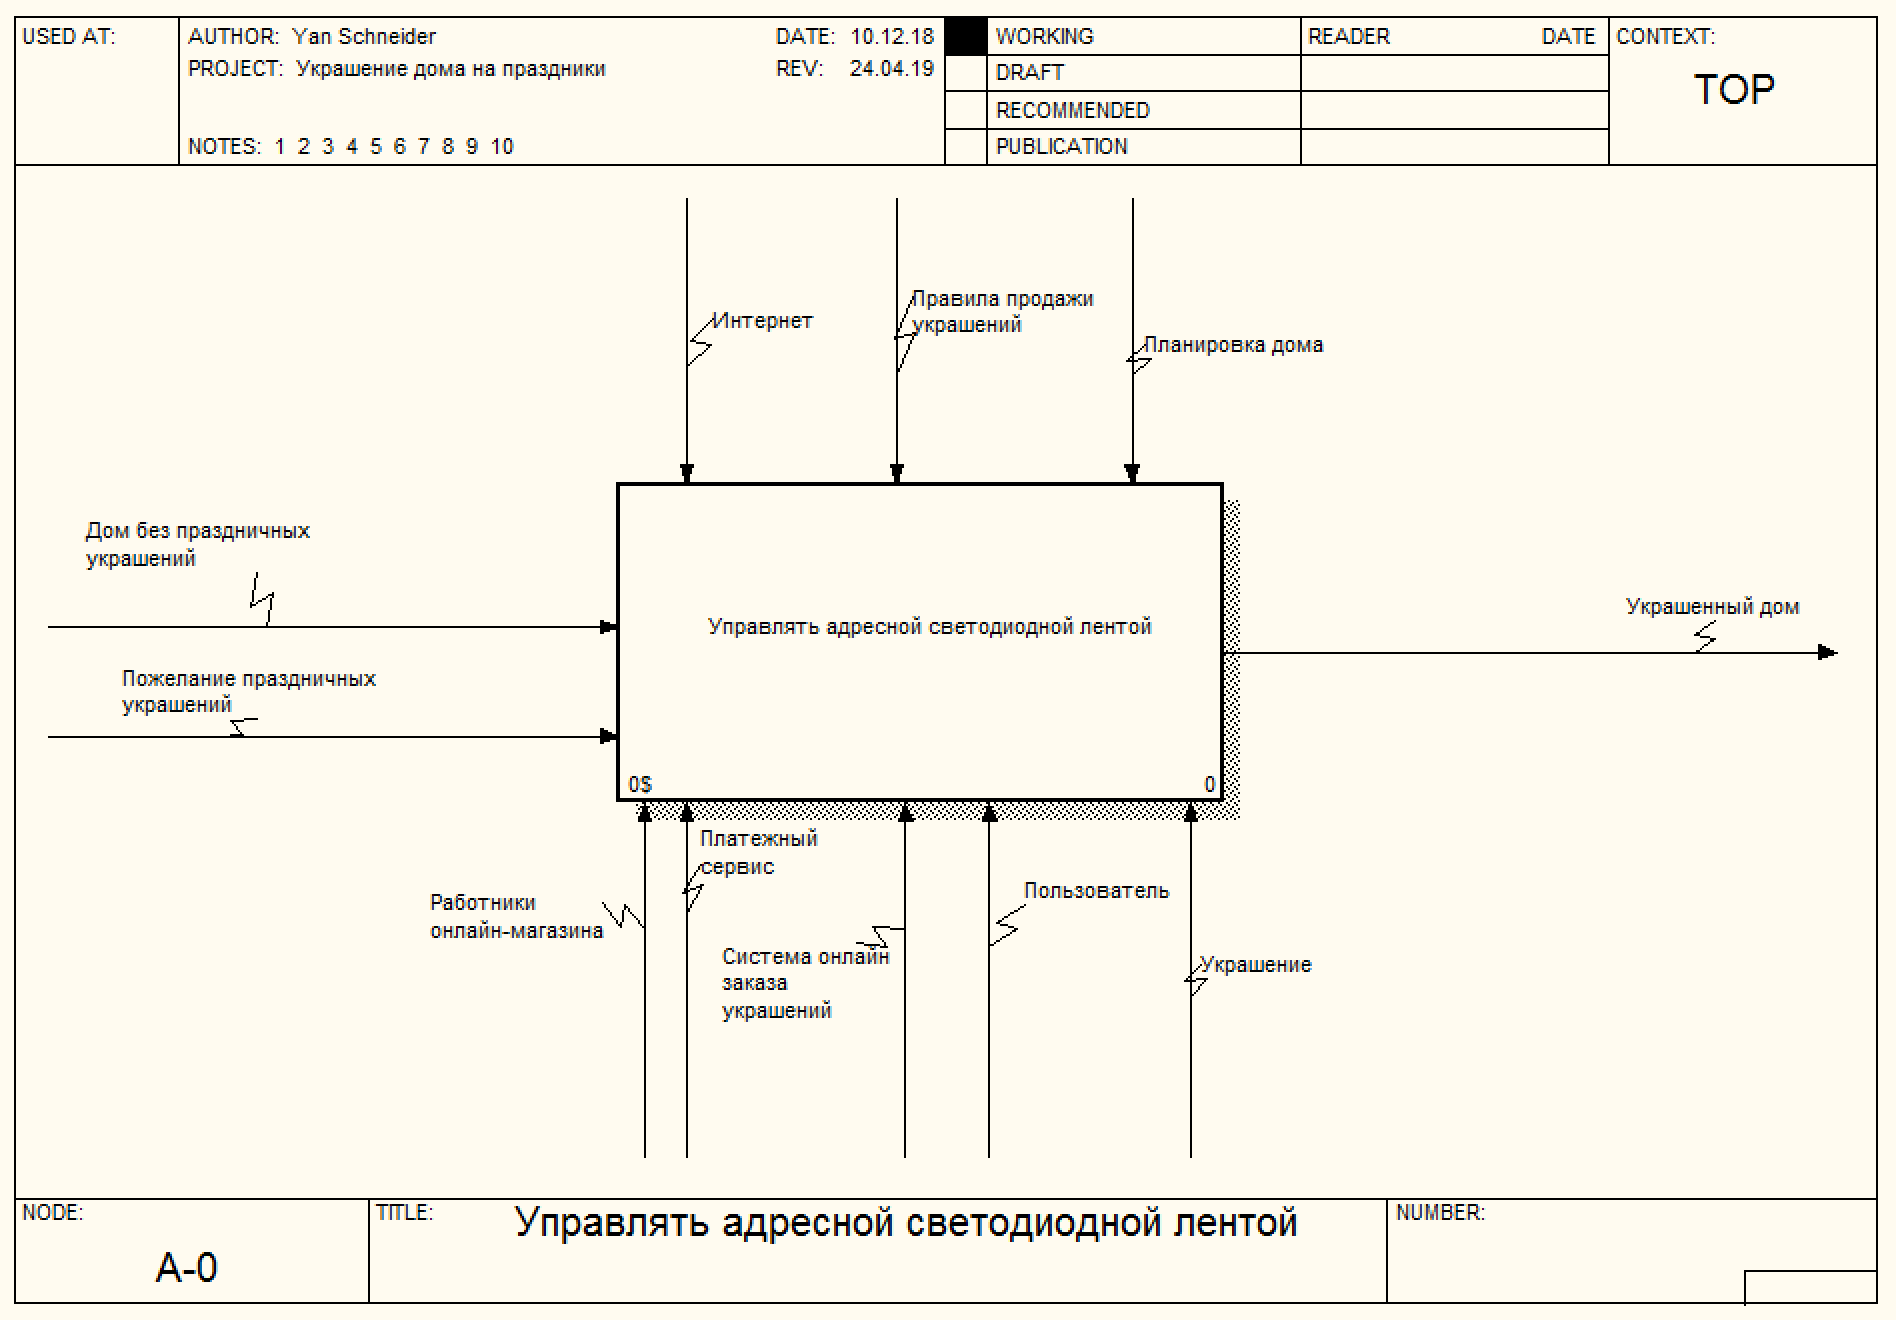
\includegraphics[scale=0.45]{figures/functionalModel/main.png}
	\caption{Контекстная диаграмма процесса управления адресной светодиодной лентой}
	\label{fig:analysis:functionalModel:main}
\end{figure}

На рисунке~\ref{fig:analysis:functionalModel:main} представлена контекстная диаграмма верхнего уровня, входными данными для которой являются дом без украшений и пожелания к ним. В рамках процесса на выходе получается украшенный дом. 

К механизмам управления относятся Интернет, правила продажи украшений и планировка дома пользователя.

Механизмы, осуществляющие процесс: работник онлайн-магазина, платежный сервис, система онлайн-заказа украшений, пользователь и само украшение (адресная светодиодная лента).

Далее в соответствии со вторым и третьим принципами, распишем основное действие на уровни.

Украшение дома декомпозировано на 4 блока: поиск, покупка, установка и настройка украшений.

Функциональная модель управления адресной светодиодной лентой показана на рисунке~\ref{fig:analysis:functionalModel:a0_decoration}.

~
\begin{figure}[H]
\centering
	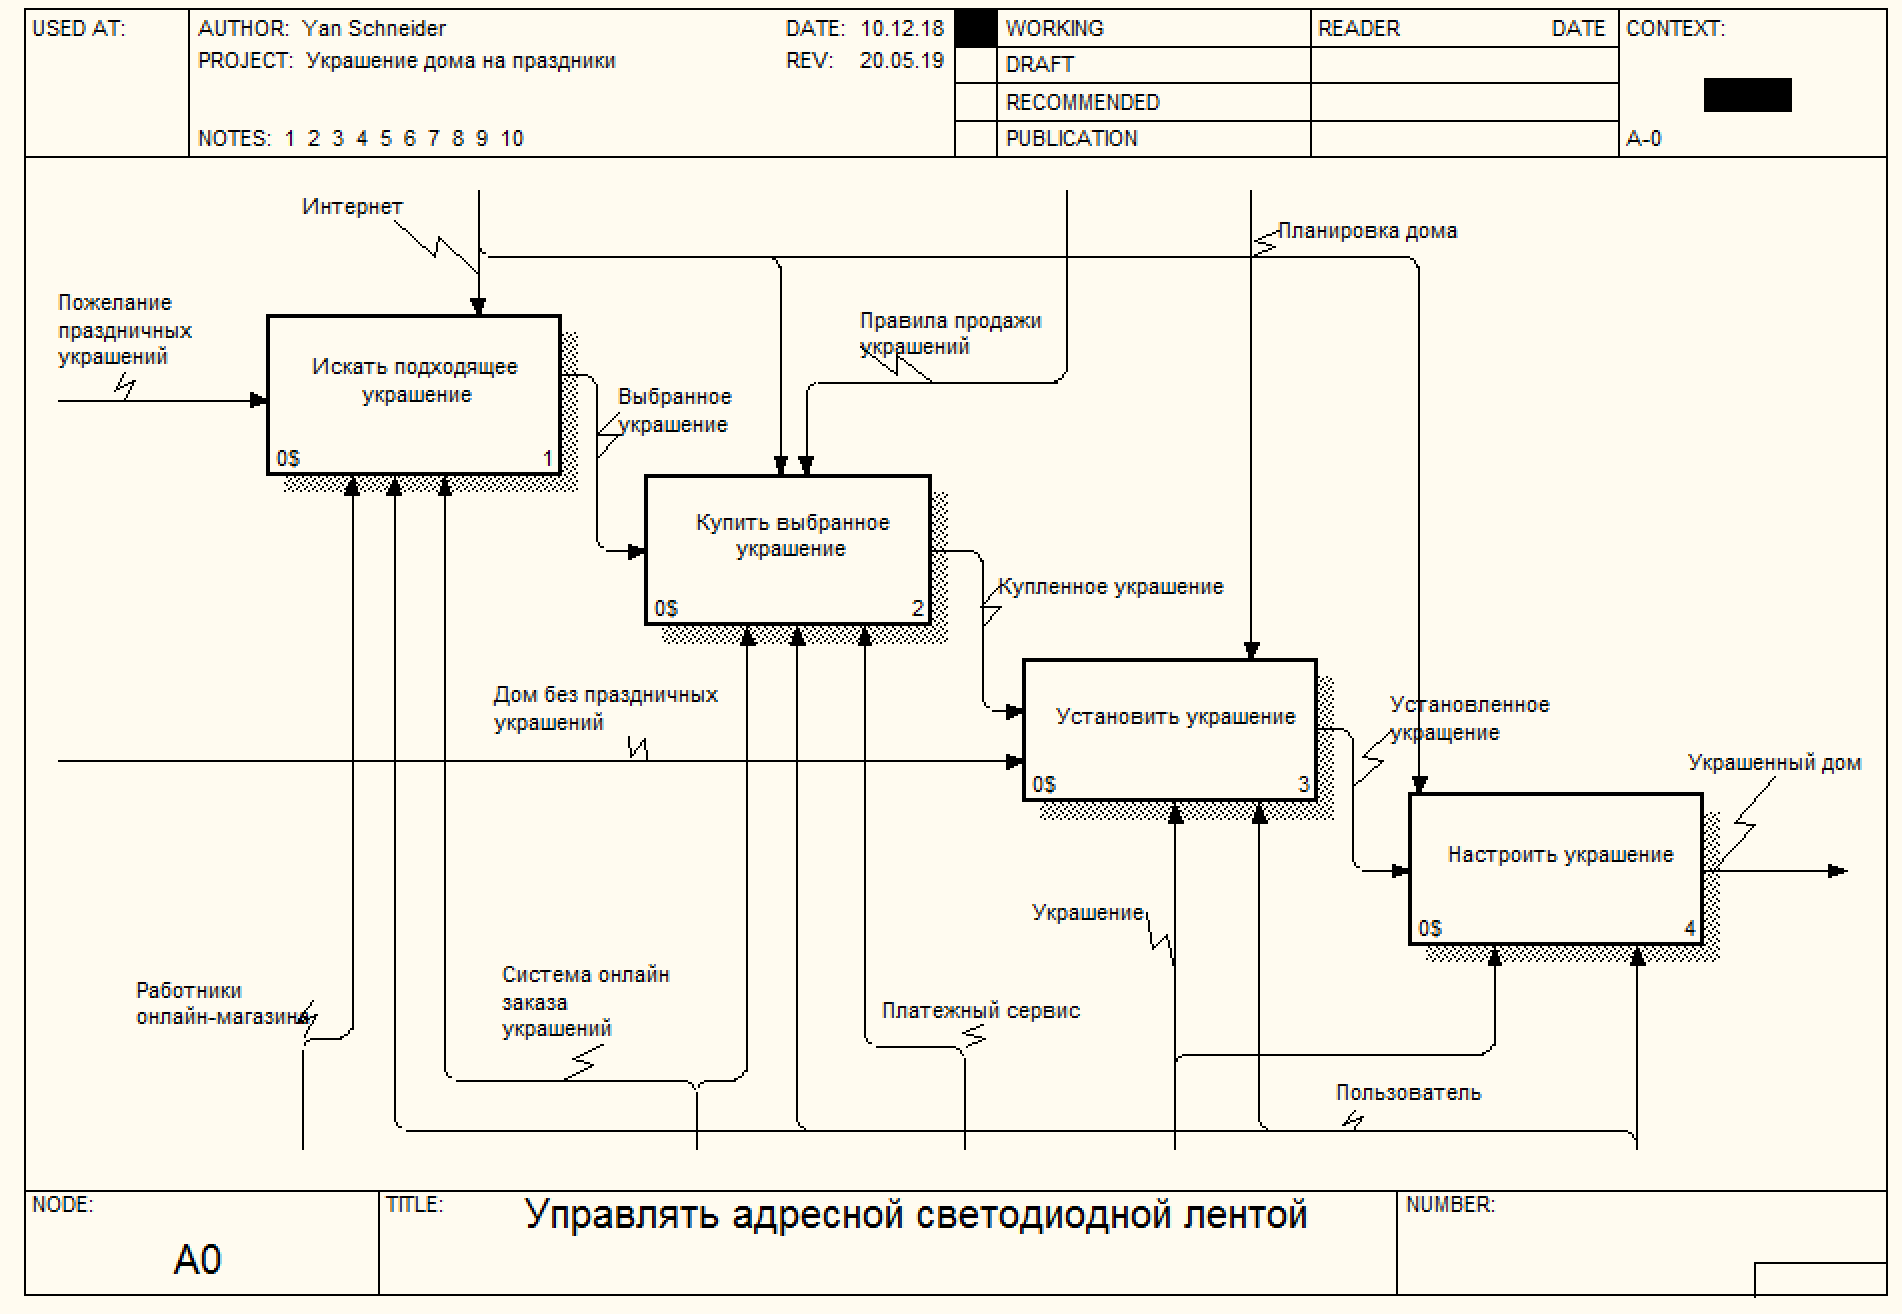
\includegraphics[scale=0.45]{figures/functionalModel/a0_decoration.png}
	\caption{Декомпозиция блока \enquote{Управлять адресной светодиодной лентой}}
	\label{fig:analysis:functionalModel:a0_decoration}
\end{figure}

Рассмотрим последовательно каждый блок.

Первый блок (рисунок~\ref{fig:analysis:functionalModel:a1_search}):

Данный блок необходим для поиска подходящего украшения для дома. Данный процесс включает в себя вход в онлайн магазин, установку фильтров для поиска, просмотр результатов поиска, консультация с работником онлайн-магазина (для дополнительной фильтрации списка выбранных украшений) и, наконец, выбор подходящего варианта.

 ~
\begin{figure}[H]
\centering
	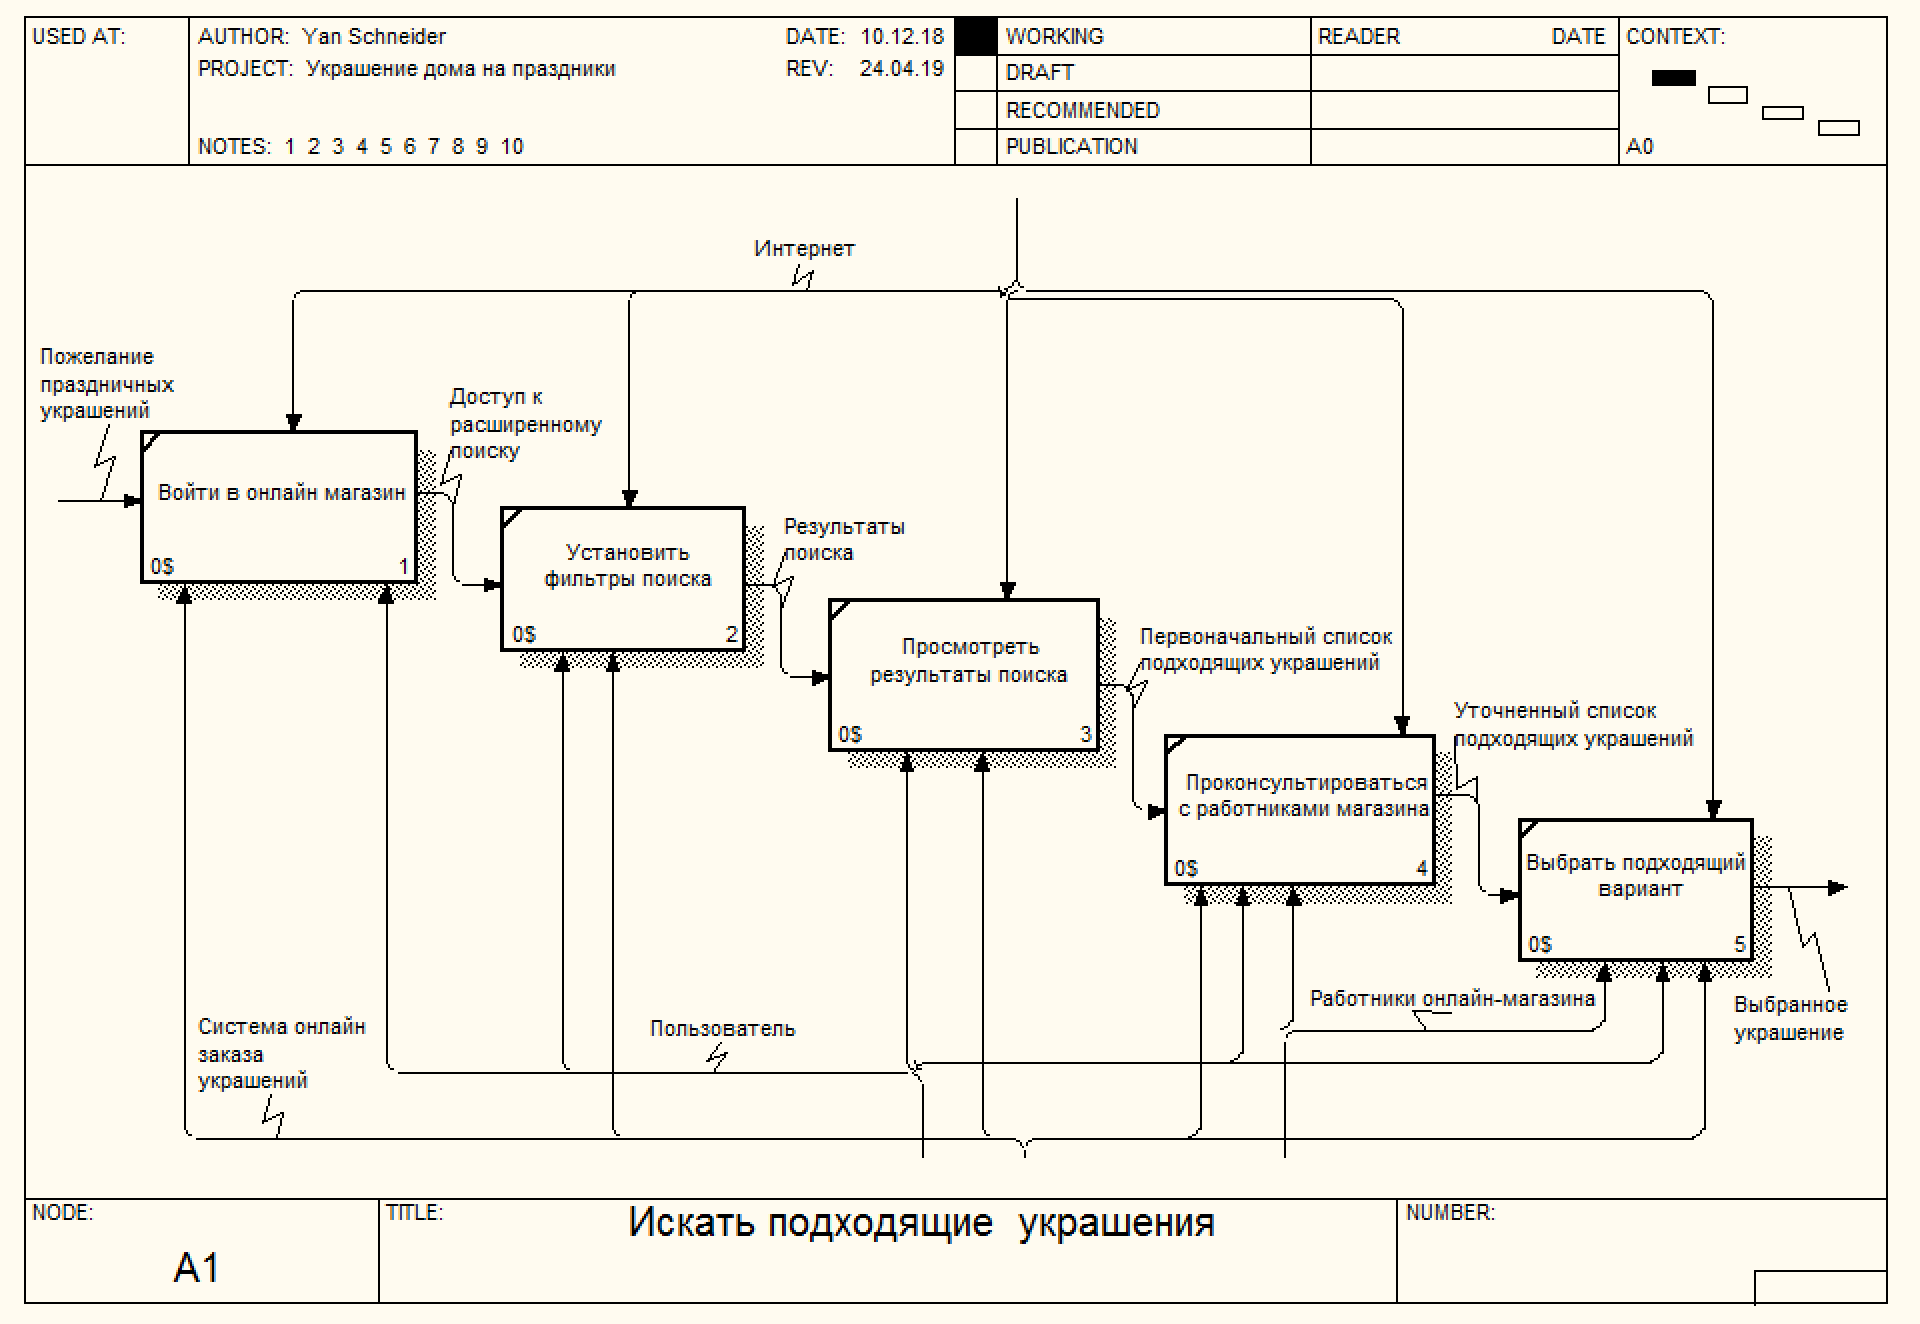
\includegraphics[scale=0.45]{figures/functionalModel/a1_search.png}
	\caption{Декомпозиция блока \enquote{Искать подходящие украшения}}
	\label{fig:analysis:functionalModel:a1_search}
\end{figure}

Второй блок представлен на рисунке~\ref{fig:analysis:functionalModel:a2_buy}. Данный блок включает в себя добавление заказа (украшения) в корзину, ввод платежной информации, ввод информации о доставке (адрес, индекс и т.д.) и оплата товара.

 ~
\begin{figure}[H]
\centering
	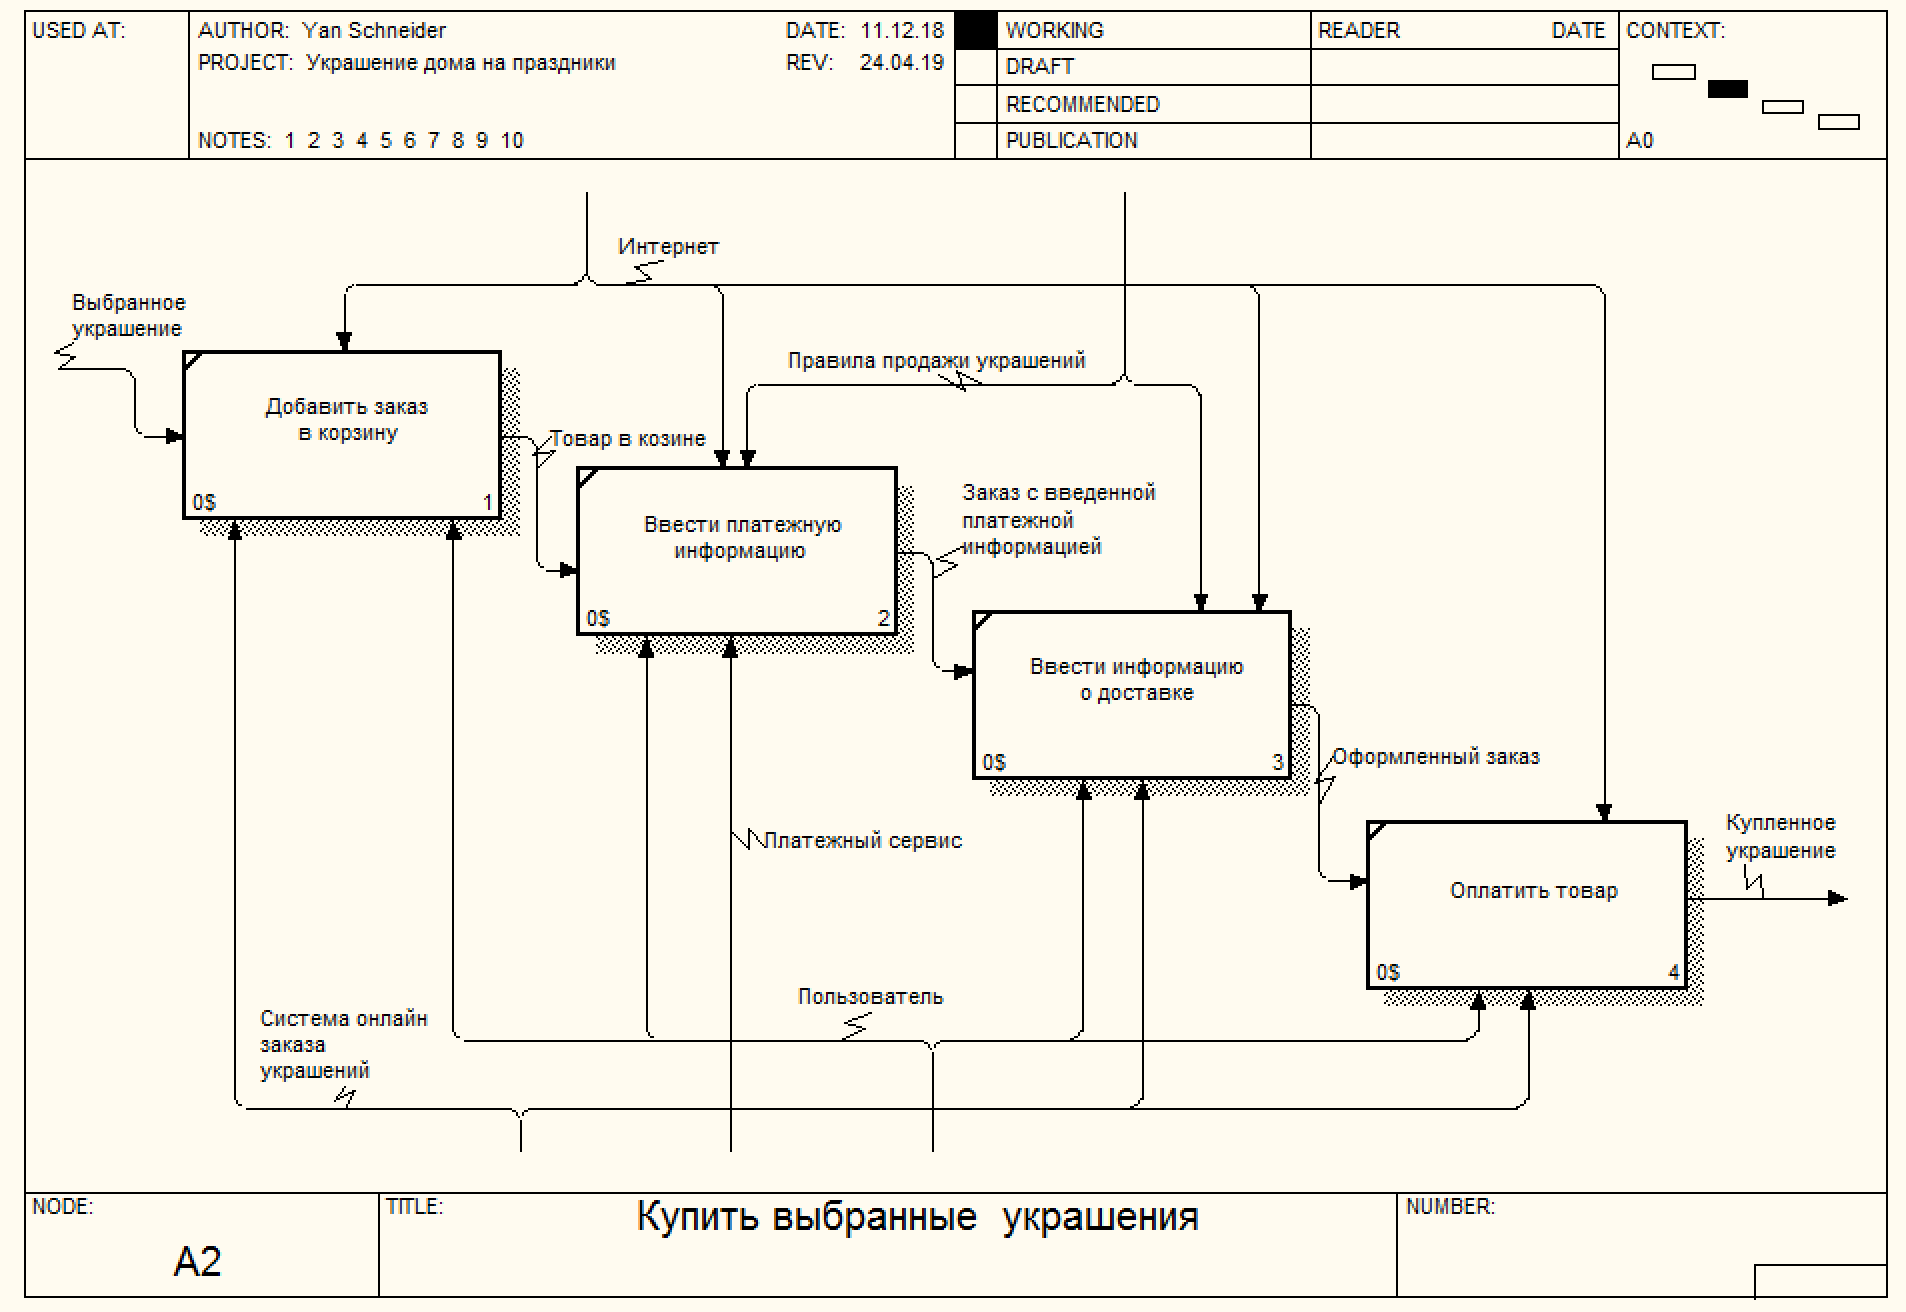
\includegraphics[scale=0.45]{figures/functionalModel/a2_buy.png}
	\caption{Декомпозиция блока \enquote{Купить выбранные украшения}}
	\label{fig:analysis:functionalModel:a2_buy}
\end{figure}

 ~
\begin{figure}[H]
\centering
	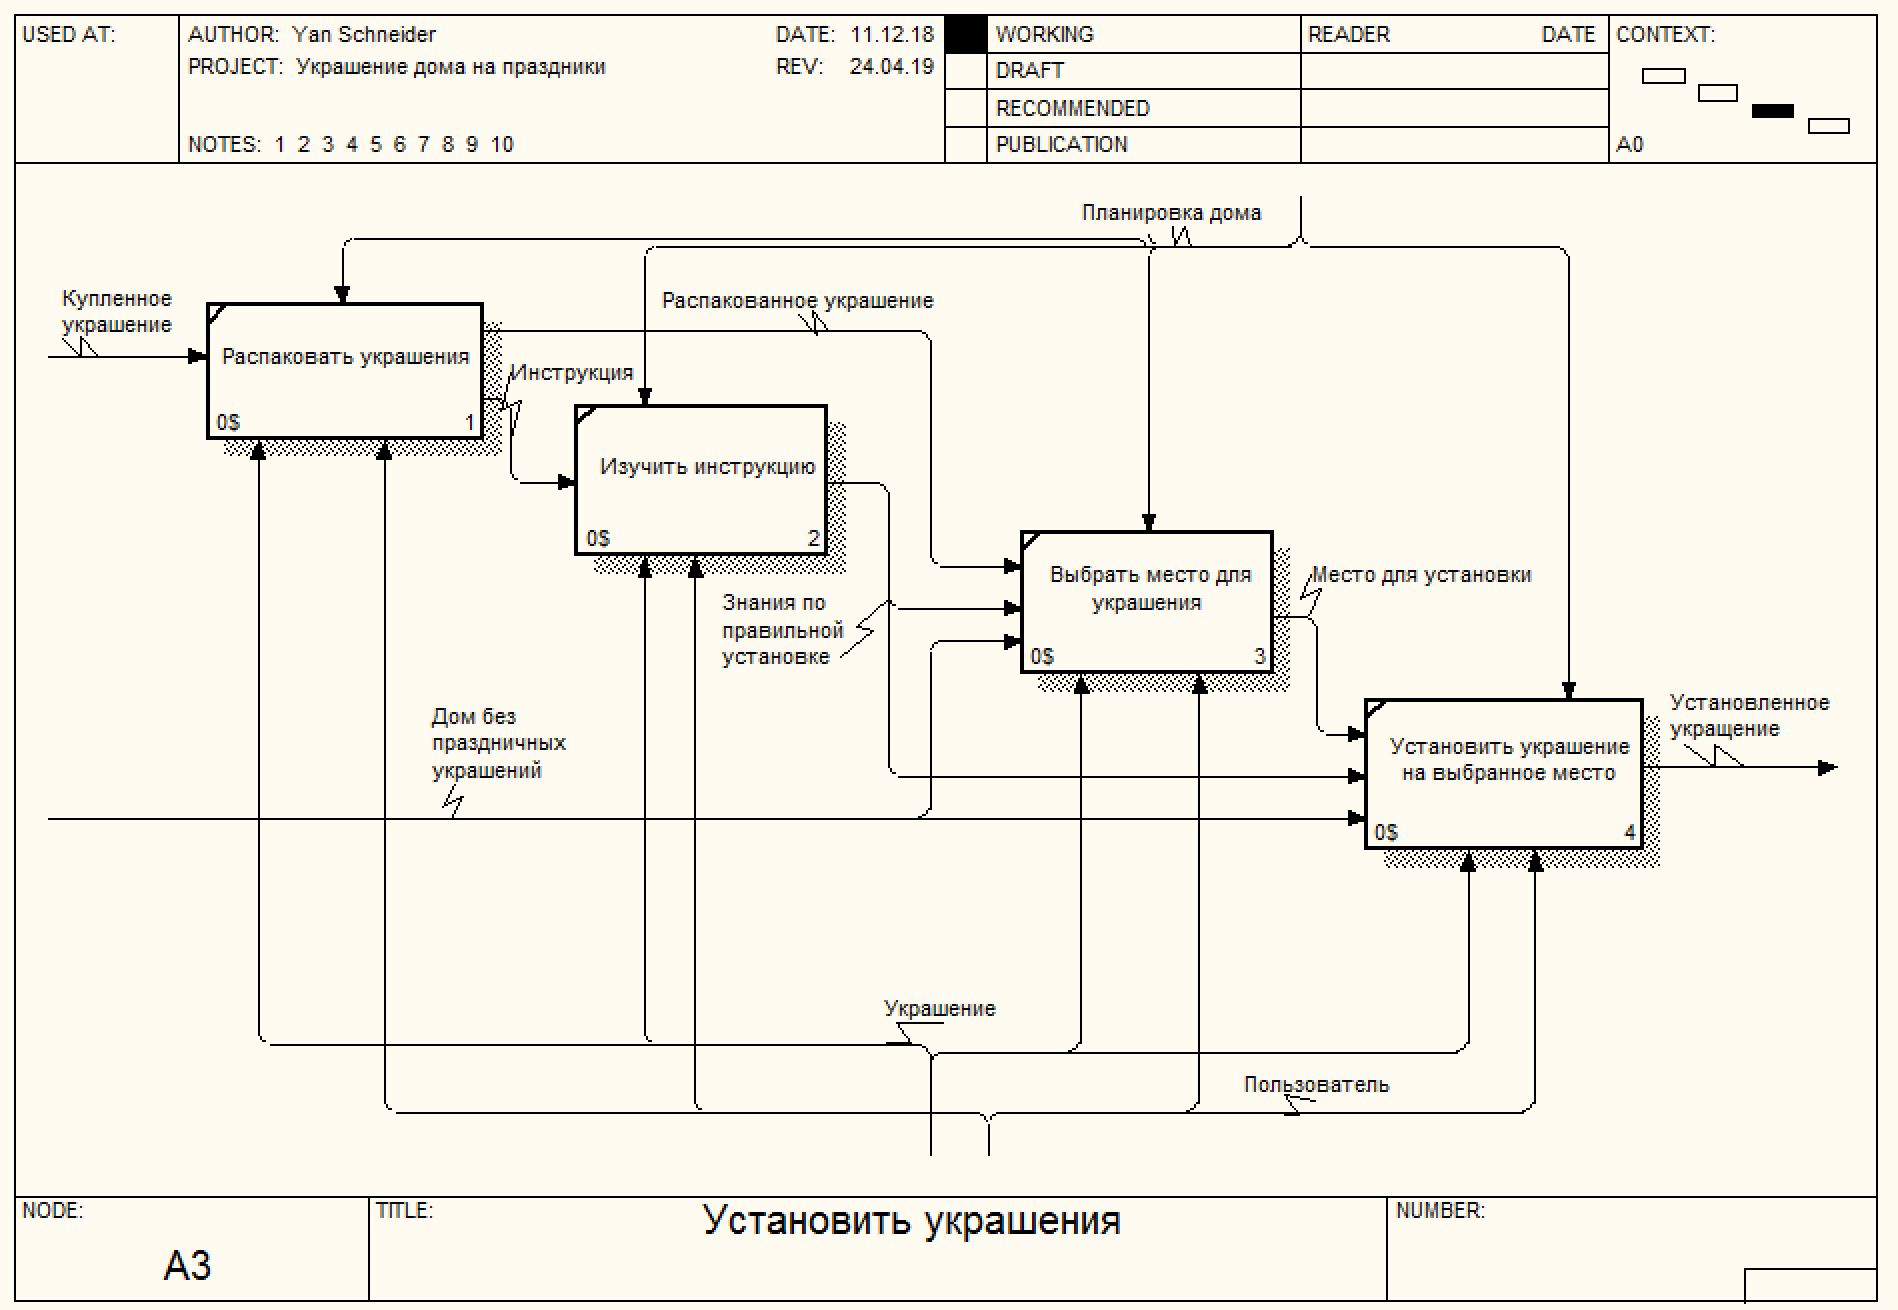
\includegraphics[scale=0.45]{figures/functionalModel/a3_install.png}
	\caption{Декомпозиция блока \enquote{Установить украшения}}
	\label{fig:analysis:functionalModel:a3_install}
\end{figure}

Третий блок (рисунок~\ref{fig:analysis:functionalModel:a3_install}):

Данный блок описывает процесс установки купленного украшения в доме. Данный процесс включает в себя распаковку украшения, чтение инструкции, выбор места для украшения и его установка.

 ~
\begin{figure}[H]
\centering
	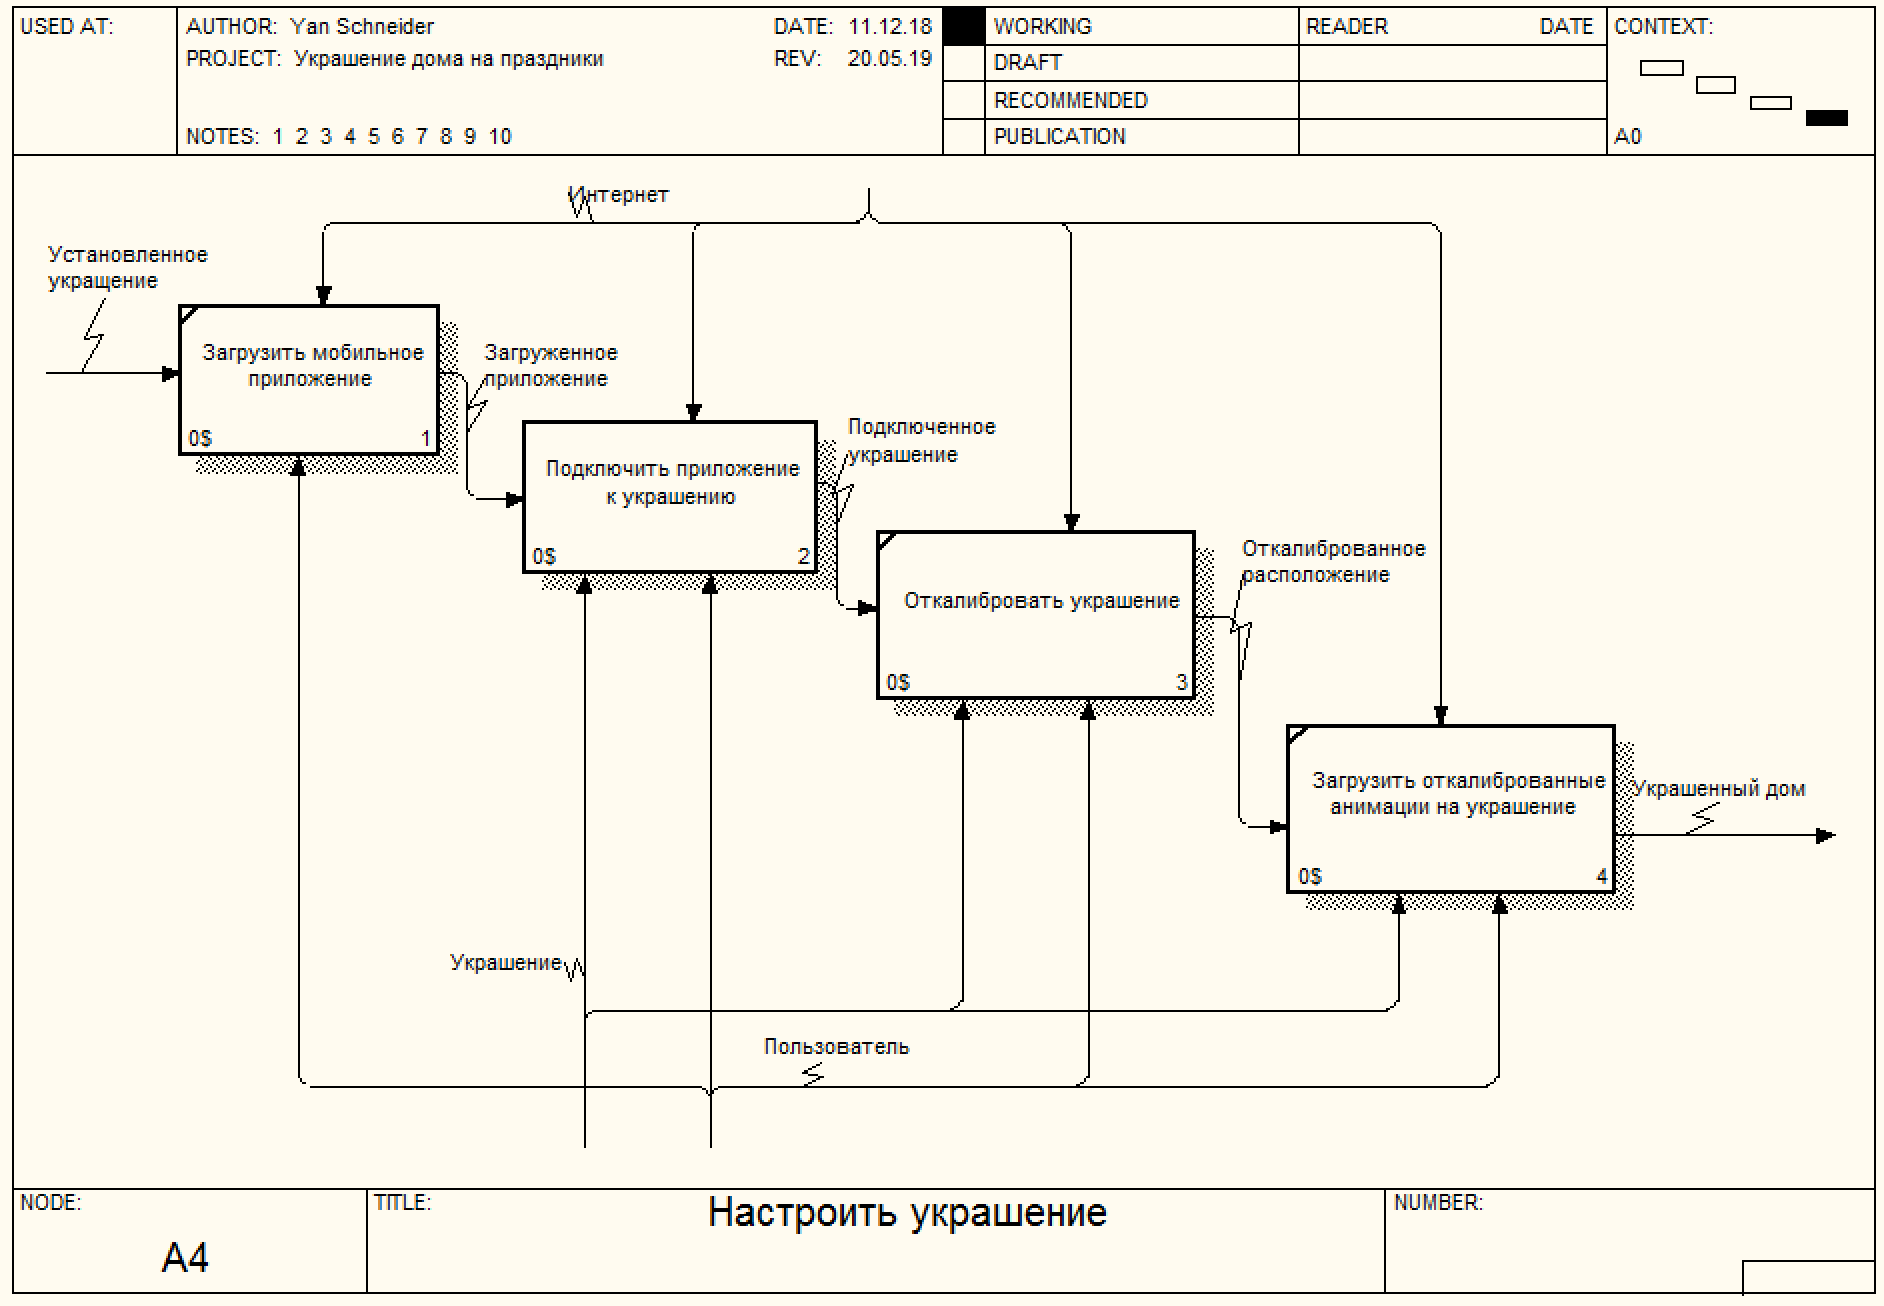
\includegraphics[scale=0.45]{figures/functionalModel/a4_settings.png}
	\caption{Декомпозиция блока \enquote{Настроить украшения}}
	\label{fig:analysis:functionalModel:a4_settings}
\end{figure}

Четвертый блок (рисунок~\ref{fig:analysis:functionalModel:a4_settings}):

Данный блок описывает процесс настройки украшений. Данный процесс включает в себя загрузку приложения для управления украшениями, подключение их к приложению, калибровку и отправку уже откалиброванных анимаций на украшения. 

~
\begin{figure}[H]
\centering
	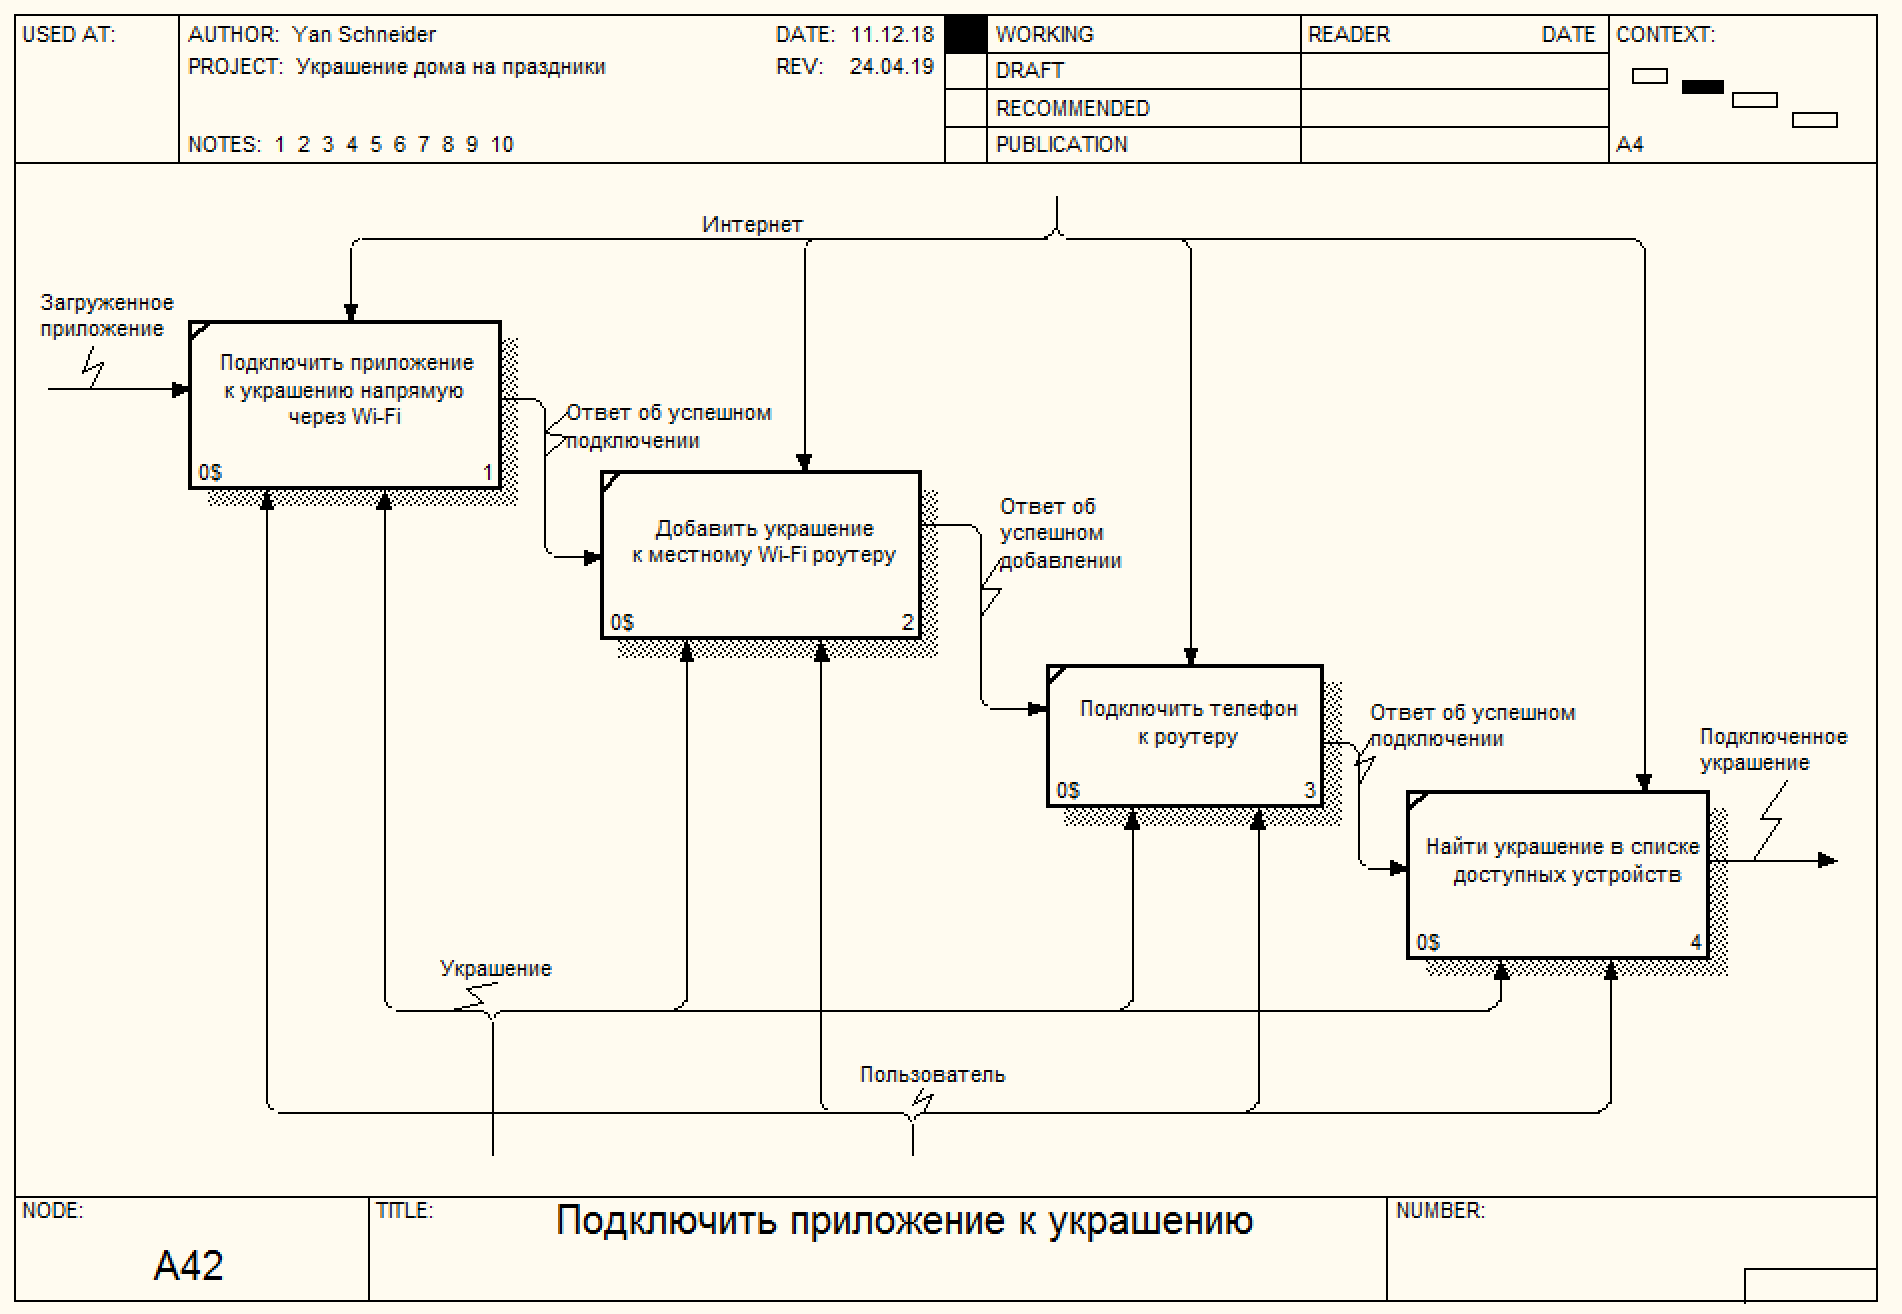
\includegraphics[scale=0.45]{figures/functionalModel/a42_connecting.png}
	\caption{Декомпозиция блока \enquote{Подключить приложение к украшению}}
	\label{fig:analysis:functionalModel:a42_connecting}
\end{figure}

Декомпозиция четвертого блока (рисунок~\ref{fig:analysis:functionalModel:a42_connecting}):

Данная декомпозиция подробнее рассматривает процесс подключения мобильного приложения к украшению (украшениям). Она разбивает данный процесс на следующие компоненты: подключение напрямую к украшению через Wi-Fi, добавление украшения к местному роутеру (ввод пароля к точке). Затем идет процес подключения украшения к роутеру. После всего следует поиск украшения в списке доступных устройств.